\documentclass[a4paper,twoside]{article}

\usepackage{epsfig}
\usepackage{subfigure}
\usepackage{calc}
\usepackage{amssymb}
\usepackage{amstext}
\usepackage{amsmath}
\usepackage{listings}
\usepackage{amsthm}
\usepackage{multicol}
\usepackage{pslatex}
\usepackage[table]{xcolor}
\usepackage{rotating}
%\SetKw{Kw}{create}
\usepackage{float}
\usepackage{multirow}
\usepackage{apalike}
\usepackage{SCITEPRESS}
\usepackage[small]{caption}
\usepackage{tikz}
\newcommand*\circled[1]{\tikz[baseline=(char.base)]{
  \node[shape=circle,draw, inner sep=0.1pt] (char) {#1};}
}

\newcommand{\tikzcircle}[2][black,fill=black]{\tikz[baseline=-0.5ex]\draw[#1,radius=#2] (0,0) circle ;}%
\lstset{language=Java,captionpos=b,tabsize=3,frame=lines,keywordstyle=\color{black},commentstyle=\color{darkgreen},stringstyle=\color{black},numbers=left,numberstyle=\tiny,numbersep=5pt,breaklines=true,showstringspaces=false,basicstyle=\footnotesize,emph={label}}

\subfigtopskip=0pt
\subfigcapskip=0pt
\subfigbottomskip=0pt

\begin{document}

\title{Authors' Instructions  \subtitle{Preparation of Camera-Ready Contributions to SCITEPRESS Proceedings} }

\author{\authorname{First Author Name\sup{1}, Second Author Name\sup{1} and Third Author Name\sup{2}}
\affiliation{\sup{1}Institute of Problem Solving, XYZ University, My Street, MyTown, MyCountry}
\affiliation{\sup{2}Department of Computing, Main University, MySecondTown, MyCountry}
\email{\{f\_author, s\_author\}@ips.xyz.edu, t\_author@dc.mu.edu}
}

\keywords{The paper must have at least one keyword. The text must be set to 9-point font size and without the use of bold or italic font style. For more than one keyword, please use a comma as a separator. Keywords must be titlecased.}

\abstract{\underline{Background:} The several maintenance tasks a system is submitted during its life usually cause its architecture deviates from the original conceived design. Therefore software engineers need processes for recovering the knowledge embedded in legacy systems in order to get both better software comprehension and software modernization. In this context, refactoring can be applied in a legacy system to do so and yet to clean up, to improve and to raise the level of reuse of the legacy system.  Refactoring is the process of changing a software system in such a way that it does not alter the external behavior of the source-code yet improves its internal structure. Nowadays, with the advent of ADM (Architecture-driven modernization), an OMG (Object Management Group) standard for modernizing legacy software systems, the refactoring process follows a  MDD (Model-Driven Development) approach using the KDM (Knowledge Discovery Metamodel) specification as the cornerstone of the standard. \underline{Problem:} we should put the problem here. \underline{Objectives:} This paper seeks to define ..... \underline{Method:} .......   
\underline{Results:} To provide some evidence of our approach....., we conducted a case study. .....
}

\onecolumn \maketitle \normalsize \vfill

\section{\uppercase{Introduction}}
\label{sec:introduction}

\noindent Software systems are considered legacy when their maintenance costs are raised to undesirable levels but they are still valuable for organizations. However, they can not be discarded because they incorporate a lot of embodied knowledge due to years of maintenance and this constitutes a significant corporate asset. As these systems still provide significant business value, they must then be modernized/re-engineered so that their maintenance costs can be manageable and they can keep on assisting in the regular daily activities. 

The first task that must be performed in order to carrying out a software modernization is understand the legacy system. It is not a trivial task, in fact studies estimate that between $50$ percent and $90$ percent of software maintenance involves developing an understanding of the software being maintained~\cite{Tilley95perspectiveson}, thus several approaches have been developed to support software engineers in the comprehension of systems where reverse engineering (RE) is one of them~\cite{Canfora2011}. RE supports program comprehension by using techniques that explore the source code to find relevant information related to functional and non-functional features~\cite{chikofskyTax}.

In this context, OMG (Object Management Group) has employed a lot of effort to define standards in the modernization process, creating the concept of ADM (Architecture-Driven Modernization). ADM follows the MDD (Model-Driven Development)~\cite{Ulrich:2010:IST:1841736}~\cite{5440163} guidelines and comprises two major steps. Firstly a reverse engineering is performed starting from the source code and a model instance (PSM) is created. Next successive refinements (transformations) are applied to this model up to reach a good abstraction level (PSM or CIM) in model called KDM (Knowledge Discovery Metamodel). Upon this model, several refactorings, optimizations and modifications can be performed in order to solve problems found in the legacy system. Secondly a forward engineering is carried out and the source code of the modernized target system is generated again. According to the OMG the most important artifact provided by ADM is the KDM metamodel, which is a multipurpose standard metamodel that represents all aspects of the existing IT (Information  Technology) architectures. The idea behind the standard KDM is that the community starts to create parsers from different languages to KDM. As a result everything that takes KDM as input can be considered platform and language-independent. For example, a refactoring catalogue for KDM can be used for refactoring systems implemented in different languages. 

\section{\uppercase{Motivation}}

\noindent Our motivation is fourfold. Firstly, is the present lack of a fully developed idea of ``good'' modernization by using ADM and its metamodels by using design patterns to assist the modernization of legacy systems. This is an important issue, for a clear notion of style is a fundamental prerequisite for the use of modernization by means of ADM, enabling programmers to see where they are heading when modernizing their legacy system. 

%A second hurdle - both a cause and a consequence of the first - is the present lack of an ADM equivalent of such catalogues. Our work is based on the assumption that the process of modernization by using KDM would equally benefit from KDM specific catalogues of smells and refactorings, helping programmers to detect situations in the KDM model that could be improved and guiding them through the corresponding transformation processes.

%Secondly, is that generally, the source code is the only available artifact of the legacy software. By applying model-based modernization, both the legacy software and the generated software will have a new type of artifact, improving their documentation. Our work is based on the assumption that the process of modernization by using ADM would equally benefiting and helping programmers to modernize a legacy systems by using its metamodels.


Secondly, one problem with automated restructuring techniques that modify source-code is that they do not restructure in-line documentation (i.e., program documentations) along with the source-code. This means that manual labor to restructure documentation is nearly always needed after applying a restructuring approach. In addition, the source-code is the only available artifact of the legacy software. We argue that by applying model-base modernization, both the legacy software and the generated software will have either a restructure documentation or a new type of artifact as result improving their documentation.

%One problem with automated restructuring techniques that modify code is they don’t restructure in-line documentation (i.e., rewrite program comments) along with the code. This means that manual labor to restructure documentation is nearly always needed after applying a restructuring approach. Automat- ing the restructuring of documentation is important for making restructuring more cost- effectiv

Thirdly, we claim that unlike the code-based modernization, model-based ones are platform independent. Thus, models can be transformed and good designs can be produced regardless of programming language. 

Finally, the absence of tool that supporting modernization by using the KDM specification in current integrated development environments. We argue that efficient tool can bring benefits to assist software engineer during the modernization process. Therefore, we also devised a proof-of-concept Modernization-Integrated Environment (MIE), which is an environment that modernizing a legacy system to services by using ADM and its metamodels.

\section{\uppercase{Background}}

\noindent In this section we provide a brief background to Architecture-Driven Modernization (ADM) presenting the core ideas. Furthermore, this section describes the an of the ADM standards, e.i., Knowledge Discovery Metamodel (KDM).

\subsection{Model-Driven Development}

Software systems are becoming increasingly complex as customers demand richer functionality delivered in ever shorter timescales~\cite{550}. 
In this context, Model-Driven Development (MDD) can be used to speed up software development and manage complexity is to shift from programming in solution-space in order to model problem-space.

MDD is an approach to software development that give particular emphasis upon making models the primary development artifact and subjecting such models to a refinement process, by using automatic transformations, until a running system is obtained. In this context, MDD aims to provide higher level of abstraction in development of systems which further results in an improved understanding of complex systems~\cite{1296153}. 

Furthermore, MDD handles problems in software systems development that originate from existence of heterogeneous platforms. It achieves this through keeping different levels of model abstractions; and by transforming models from Platform Independent Models (PIMs) to Platform Specific Models (PSMs). Therefore, automatic  generation of application code (i.e. automatic model-driven code generation) offers many advantages such as the rapid development of high quality code, reduced number of accidental programming errors, enhanced consistency between design and code~\cite{Schmidt06_ModelDrivenEngineering}. Changes in implementation strategies can be achieved through modifying the transformations. Shifting engineering concerns to platform-independent levels allows developers to focus on designing applications without involvement in platform-specific concepts.

It is worth highlight that models in MDD are usually represented by domain-specific languages~\cite{Fowler:2010:DSL:1809745}, i.e., a language that adequately represents the information of a given domain. Instead of representing elements using a general purpose language, producing source code (e.g., Java) and class diagrams (e.g., plain UML models), the knowledge is described in a language which the domain experts understand. Besides, as the expert uses a suitable language to describe the system at hand, the accidental complexity that one inherent from the restrictions of the language to properly describe a given domain is reduced, leaving only the essential complexity of the problem. 

\subsection{Architecture-Driven Modernization}

Nowadays, researchers have been shifted from the typical refactoring process to the so-called Architecture-Driven Modernization (ADM). ADM is the concept of modernizing existing systems with a focus on all aspects of the current systems architecture and the ability to transform current architectures to target architectures by using all principles of MDD~\cite[p.~60]{Ulrich:2010:IST:1841736}. Figure~\ref{horseshoe} shows the ADM modernization domain model where the left side of the horseshoe is the current state of a business architecture ``as-is'' and the right side is what we want to get after the modernization ``to-be''.


\begin{figure}[!ht]
\centering
  % Requires \usepackage{graphicx}
  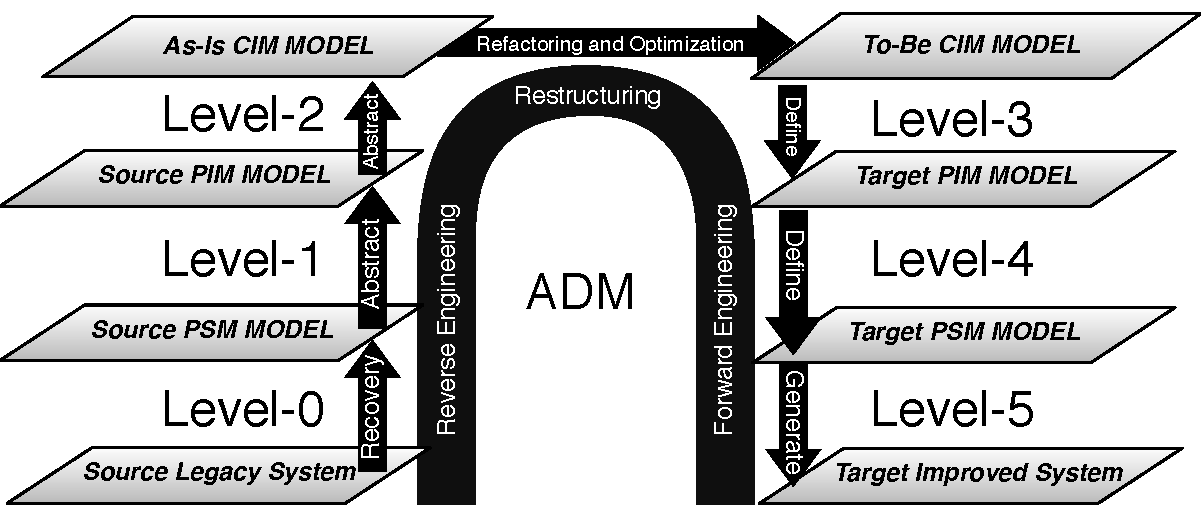
\includegraphics[scale=0.37]{figuras/Fonte_horse_shoe}
\caption{Modernization domain model (Adapted from Ulrich and Newcomb~\cite{Ulrich:2010:IST:1841736})}
\label{horseshoe}
\end{figure}

As can be seen in Figure~\ref{horseshoe} the horseshoe reengineering model has been adapted to ADM and it is nowadays known as horseshoe modernization model. As ADM uses the principles of MDD three kinds of models in the horseshoe are used, they are: (\textit{i}) PIM - \textbf{P}lataform \textbf{I}ndependent \textbf{M}odel which represents a view of the system from the platform independent viewpoint at an intermediate abstraction level, (\textit{ii}) PSM - \textbf{P}lataform \textbf{S}pecific \textbf{M}odel which constitutes a view of the system from the platform specific viewpoint at a low abstraction level, and (\textit{iii}) CIM - \textbf{C}omputational \textbf{I}ndependent \textbf{M}odel that represents a view of the system from the computational independent viewpoint at a high abstraction level. These models are used in the steps of the ADM process, i.e., Reverse Engineering, Restructuring, and Forward Engineering. In the first step, a reverse engineering is performed starting from the artifacts of the legacy system (source code, database, configuration files, etc) and a set of PSM are created. Next, refactoring and restructuring techniques can be applied on these models in order to solve problems found in the legacy system. Therefore, this step consist of a set of transformation from the input model (``as-is'') to obtain a target model (``to-be''). Finally, a forward engineering is carried out and the source code of the modernized target system is generated again. 


In order to perform such steps, ADM introduces several modernization standards: Abstract Syntax Tree Metamodel (ASTM), Knowledge Discovery Metamodel (KDM), Structured Metrics Metamodel (SMM), etc. The next subsections present more information about these standards:


%System Assurance \& Evidence, Software Quality and Business Architecture Standards. Nevertheless, in this paper we are especially interested in KDM, i.e., it is the key cornerstone of ADM and KDM owns a set of metamodel elements whose purpose is to represent implementation level program elements and their associations. The details of KDM are described as follows:

\subsubsection{Knowledge Discovery Metamodel - KDM}\label{subsec:KDM}

Knowledge Discovery Metamodel (KDM) is the key within set of standards~\cite{1686216}. KDM allows standardized representation of knowledge extracted from legacy systems by means of reverse engineering. KDM provides a common repository structure that makes possible the exchange of information about existing software assets in legacy systems. This information is currently represented and stored independently by heterogeneous tools focused on different software assets~\cite[p.~32]{Ulrich:2010:IST:1841736}. Figure~\ref{kdm} shows each of the varying views of the existing IT architecture represented by the KDM. For example, the build view, depicts system artifacts from a source, executable, and library viewpoint. Other perspectives include design, conceptual, data, and scenario views.

\begin{figure}[!ht]
\centering
  % Requires \usepackage{graphicx}
  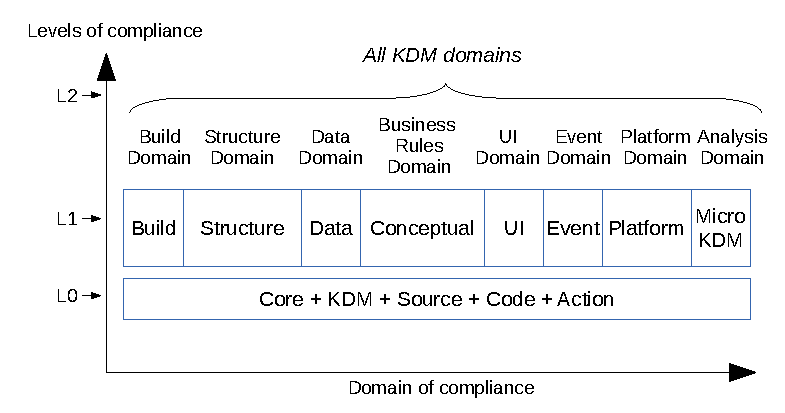
\includegraphics[scale=0.58]{figuras/kdm}
\caption{KDM domains of artifact representation (Adapted from Ulrich and Newcomb~\cite{Ulrich:2010:IST:1841736})}
\label{kdm}
\end{figure}

The Level 0 (L0) encompasses the Infrastructure and Program Elements Layer. Infrastructure Layer consists of the Core, kdm, and Source packages which provide a small common core for all other packages. Program Elements Layer consists of the Code and Action packages providing programming elements such as  data types, data items, classes, procedures, macros, prototypes, templates and captures the low level behavior elements of applications, including detailed control and data flow between statements. The Level 1 (L1) cover the Resource Layer which represents the operational environment of the existing software system. For example, the knowledge related to events and state-transition, the knowledge related to the user interfaces of the existing software system and the knowledge related to persistent data, such as indexed files, relational databases, and other kinds of data storage. The Level 2 (L2) cover the Abstraction Layer which represents domain and application abstractions. 

%As we stated earlier, herein we are only interested in the Program Element Layer - more specifically  in the Code Package, which represents the code elements of a program and their associations. Therefore, it is important to dig a little deeper in this metamodel because it is mainly used by our approach in order to identify concerns. 

%In a given KDM instance, each instance of the code meta-model element represents some programming language construct, determined by the programming language of the existing software system. Each instance of a code meta-model element corresponds to a certain region of the source code in one of the artifacts of the existing software system. In addition, the Code package consists of $24$ classes  and contains all the abstract elements for modeling the static structure of the source code. However, we are particularly interested in some of them. In Figure~\ref{fig:programLayer} is depicted a chunk of the Code package. It worth to notice that the more important metaclasses used herein are highlighted.

%\begin{figure}[!ht]
%\centering
  % Requires \usepackage{graphicx}
 % \includegraphics[scale=0.42]{figuras/ProgramLayer}
%\caption{Chunk of the Code Package (OMG Group~\cite{OMGADM})}
%\label{fig:programLayer}
%\end{figure}

%As can be seen in Figure~\ref{fig:programLayer} the root metaclass is \textit{ComputationalObject} which has two sub-metaclasses, i.e., \textit{DataElement} and \textit{ControlElement}. The former sub-metaclass, \textit{DataElement}, is a generic modeling element that defines the common properties of several concrete classes that represent the named data items of existing software systems, for example, global and local variables, record files, and formal parameters. \textit{DataElement} has five sub-metaclasses - \textit{StorableUnit}, \textit{IndexUnit}, \textit{ItemUnit}, \textit{ParameterUnit} and \textit{MemberUnit}. \textit{StorableUnit} is a concrete  sub-metaclass of the \textit{StorableElement} meta-class that represents variables of the existing software system. \textit{IndexUnit} class is a concrete subclass of the \textit{DataElement} class that represents an index of an array datatype. Instances of \textit{ItemUnit} class are endpoints of KDM data relations which describes access to complex datatypes. \textit{ParameterUnit} class is a concrete subclass of the \textit{DataElement} class that represents a formal parameter; for example, a formal parameter of a procedure. \textit{MemberUnit} class is a concrete subclass of the \textit{DataElement} class that represents a member of a class type. Finally, the latter, \textit{ControlElement} is a sub-metaclass that contains two sub-metaclasses - \textit{MethodUnit} and \textit{CallableUnit}. \textit{MethodUnit} element represents member functions owned by a \textit{ClassUnit}, including user-defined operators, constructors and destructors. The \textit{CallableUnit} represents a basic stand-alone element that can be called, such as a procedure or a function. As can be seen below the dashed line in Figure~\ref{fig:programLayer} there are also the following enumerations: ``\textit{ExportKind}'', ``\textit{StorableKind}'', ``\textit{CallableKind}'', ``\textit{MethodKind}'', which are sets os literals used as properties of the metaclasses.

 \begin{figure*}[!t]
\centering
  % Requires \usepackage{graphicx}
  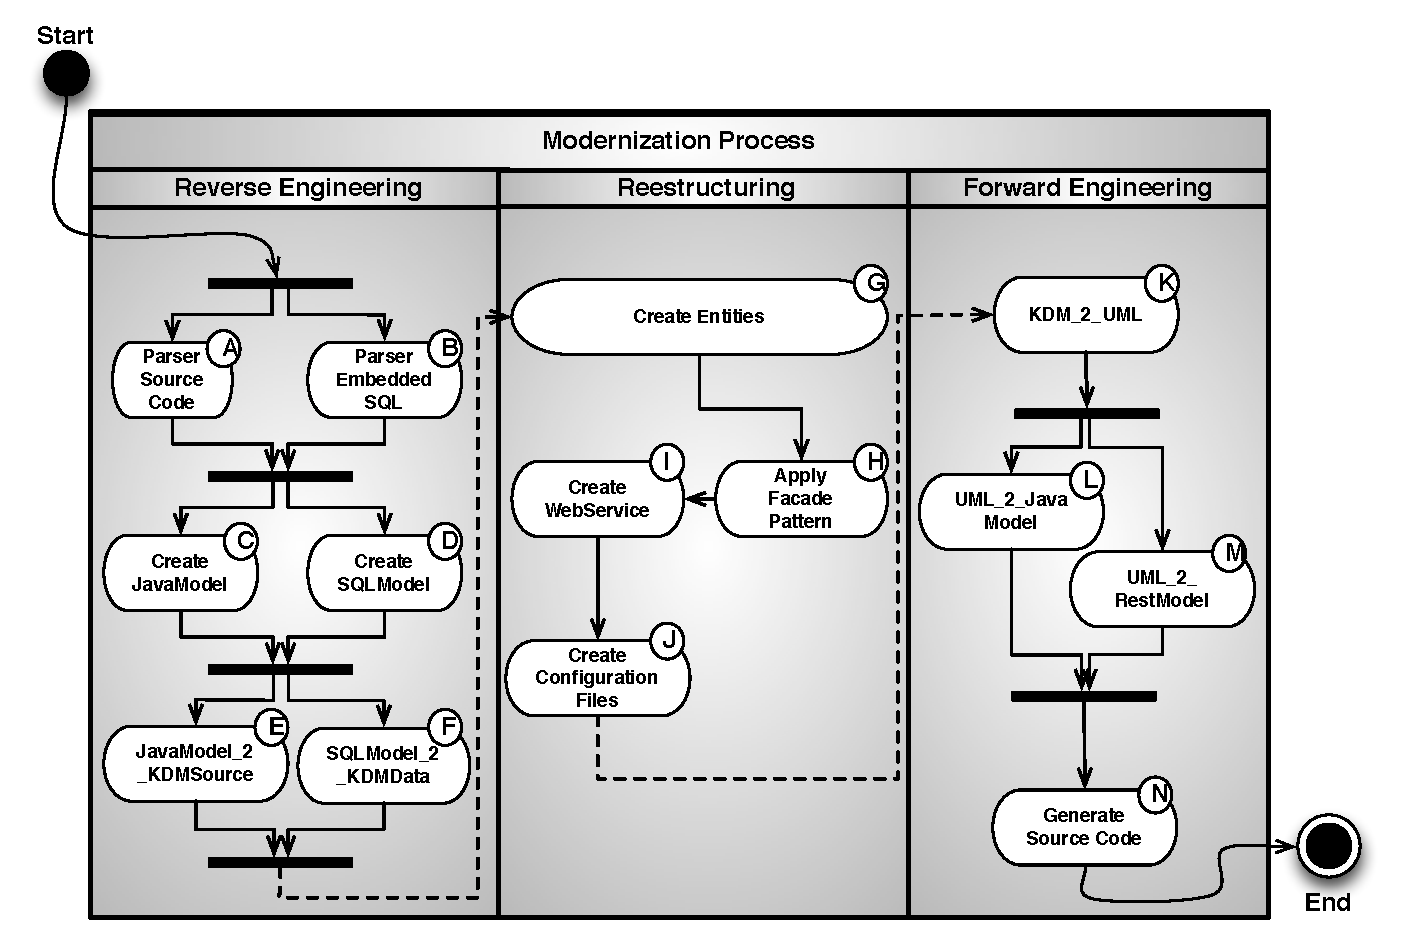
\includegraphics[width=16.8cm, height=9cm]{figuras/AllProcess4}
\caption{Modernization Activity Diagram.}
\label{fig:activity_diagram}
\end{figure*}

\section{\uppercase{Proposed Approach}}
\label{sec:proposed_approach}


\noindent By combining the concepts of software modernization, ADM and MDD, this paper proposes an approach to furnish software reengineering of legacy systems to web services. In others words, the central goal of the approach is to supply an automate way to support the modernization of legacy systems, aiming to provide reduction in time and effort spent by using code generation and to assist the migration of these systems to web services.  

We assume that a legacy systems which uses databases can decomposed into services. More specifically, our approach relies on seeking for embedded Structured Query Language (SQL) queries into the source-code of the legacy system  to restructure and re-organize the system by using design patterns, such as Facade. Then CRUDs (Create, Retrieve, Update and Delete) by using KDM are devised, i.e., services are created by means of model transformation. For example, suppose that an embedded SQL \textit{F} is found into the source-code of the legacy systems. In this case, a set of both transformations and rules are applied into this SQL, then a model \textit{F'} which contains information (table(s), column(s), relationship, etc) related to the embedded SQL \textit{F} is created. Thus, \textit{F'} is said to be equivalent to $\textit{F} \Leftrightarrow \textit{F'} $, but now \textit{F'} is represented by model. Then, this \textit{F'} is transformed into an instance of KDM and rules of modernization are applied until it reach the intended behavior, i.e., services. Finally, a forward engineering is carried out and the source code of the modernized target system is generated. 


%the approach seeks for embedded Structured Query Language (SQL) queries into the source-code of the in order to restructure and re-organize the system by using design patterns, such as Facade, then CRUDs (Create, Retrieve, Update and Delete) by using KDM, i.e., services are created by means of model transformation. 

In order to explain our approach, there is an activity diagram on Figure~\ref{fig:activity_diagram} with all steps illustrated by a capital letter inside a circle. Each step must be carry out in order to modernize the legacy systems. Moreover, this diagram consist of three main phases: (\textit{i}) Reverse Engineering (RE), (\textit{ii}) Reestructuring, and (\textit{iii}) Forward Engineering (FE). These phases are explained as follows:



\subsection{Reverse Engineering - RE} 

The aim of this phase is to analyze the legacy systems in order to identify the components of the system and their interrelationships. Furthermore, it also intends to build a set of representation of the legacy system's artifacts at a higher level of abstraction, i.e., both PSM and PIM are created in this phase. 

In our approach the RE starts by parsing two artifacts: (\textit{i}) the legacy system's source-code, and (\textit{ii}) the embedded SQL queries, Figure~\ref{fig:activity_diagram} steps \circled{\textbf{A}} and \circled{\textbf{B}}. Therefore, the  approach need to use parser to obtain information related to these artifacts. 

The former parser (see Figure~\ref{fig:activity_diagram} step \circled{\textbf{A}}) is responsible to take as input the source-code of the legacy system and then to build a data structure as output, e.g., herein the output is represented by an Abstract Syntax Tree - (AST)  which is a tree representation of the abstract syntactic structure of Java source code, by using it is possible to carry out either analysis or transformation on documents that contain programming language text.


 The latter parser (see Figure~\ref{fig:activity_diagram} step \circled{\textbf{B}}) exhaustively scans the source-code. As the parser finds an SQL statement embedded into the source-code of the legacy system, such as \textit{Select}, \textit{Delete}, \textit{Update} and \textit{Insert}, it translates those statement into an AST. As a common programming technique, many SQL statements (or partial of them) are declared as string variables, therefore variable  declarations and assignments are also of our focus.
In Listing~\ref{list:embeddedSQL} depicts a chunk of code which contains four SQL statement. 

\begin{lstlisting}[caption=Example of Embedded SQL, label=list:embeddedSQL, frame=lrtb, basicstyle=\tiny]
public class Entity {

 private String sql1 = "SELECT * FROM TABLE_1";

 public void meth() {
  String sql3 = "UPDATE TABLE3 SET column1=value1, WHERE some_column=some_value;"
  
  String sql4 = "INSERT INTO TABLE_4 VALUES (value1,value2,value3);"
  
  String sql5 = "DELETE FROM table_name WHERE some_column=some_value;"
  }
}
\end{lstlisting}





For instance, for each SQL statement, i.e., Select in line 5, Update in line 8, Insert in line 10 and Delete in line 12 the parser recognizes, analyzes and creates an AST. This AST contains information related to the name of the tables and some columns that are involved in such statements. Nevertheless, as can be seen some statements hide important informations (see Listing~\ref{list:embeddedSQL} line 5) such as the columns of a table. Therefore, initially this AST is not complete once it just owns the names of the tables and some columns. However, name of the tables and some columns are not sufficient as the approach need to identify all columns of a table, to recognize if the column is either primary key or foreign key, to pinpoint the relationships among the tables, and also to identify the type of the columns. Therefore, to address this issue the approach need to connect to the database of the legacy system in order to get these information.  As for getting this information the approach uses database metadata (data about database data). Metadata provides a structured description of database information resource and services.




%just the names of the tables and columns are not sufficient

 %since some statements do not explicitly shows the columns (see Select statement in Listing~\ref{list:embeddedSQL} line 5) and    


 %then would create an AST. It worth notice that in these statements the parser would identify just the name of the table and some columns. However, just the name of the tables are not sufficient, once the table has columns (it can be either primary key or foreign key), relationships, and also the type of the columns. Therefore, to address this issue the approach need to connect to the legacy system's database to get these information. As for getting this information the approach uses metadata API


 %Similarly, the Update, Insert and Delete statements also 

%for our approach only the tables and its columns. As can be seen in line 5 the columns are not explicitly written. Thus, in order to identify which column(s) an specifically table has the approach must connect to the legacy system's database to get this information. Furthermore,  

%the approach uses the Application Programming Interface (API)  Java DataBase Connectivity (JDBC) Metadata.









After parsing the artifacts two steps must be carry out: (\textit{i}) to create a PSM to represent the source-code of the legacy systems - the AST obtained by the first parser described aforementioned will be transformed to an instantiation of the Java meta-model, and (\textit{ii}) to create a PSM which represents the SQL identified in the source-code - the second AST obtained and described earlier will be transformed to an instantiation of an SQL meta-model, these steps are depicted in Figure~\ref{fig:activity_diagram} steps \circled{\textbf{C}} and \circled{\textbf{D}}, respectively.



%After parsing the artifacts two PSM must be obtained by mean of a set of model transformation. More specifically, the AST which represents information related to the source-code will be transformed to an instantiation of the Java meta-model. In the same way, the AST which contains information related to the embedded SQL will be transformed to an instantiation of the SQL meta-model. These are depicted in Figure~\ref{fig:activity_diagram} steps \circled{\textbf{C}} and \circled{\textbf{D}}.

In the steps \circled{\textbf{C}} a set of rules must be applied to transform the AST into a instance of the Java meta-model. 
 Java meta-model is the reflection of the Java language, as defined in version 3 of ``Java Language Specification'' from Sun Microsystems. Due space limitation in Figure~\ref{fig:java_metamodel} is depicted just a chunk of the Java meta-model; the complete Java meta-model contains 126 meta-classes. As can be seen, in Figure~\ref{fig:java_metamodel} each meta-classes is intended to represent an element of the Java language. For instance, each ``package'' found in the source-code is transformed to instances of the meta-classe ``Package'', ``Classes'' are transformed to instances of the meta-classe ``ClassDeclaration'', ``Fors'' are transformed to instances of the meta-classe ``ForStatement'', etc;

\begin{figure}[!h]
\centering
  % Requires \usepackage{graphicx}
  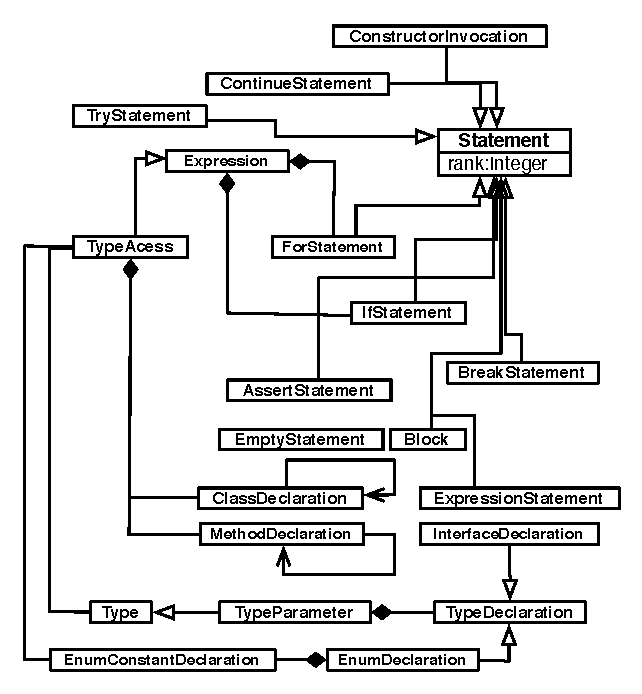
\includegraphics[scale=0.74]{figuras/JavaMOdelNovo}
\caption{Java meta-model (simplified excerpt).}
\label{fig:java_metamodel}
\end{figure}

On the fourth step (see Figure~\ref{fig:activity_diagram} \circled{\textbf{D}}) an instance of the SQL model must be obtained. The SQL model used herein is represented in a PSM model according to the SQL-92 standard (ref). Figure~\ref{fig:sql_metamodel} presents the SQL meta-model. This meta-model contains meta-classes to represent each element identified by the second parser. More specifically, the tables identified earlier (rule R1), its columns (rule R2), the data type associated with each column (rule R3), the primary key associated with each table (rule R4), and the foreign key associated with each table (rule R5) is represented by this meta-model. Next, we describe each of these rules.

\begin{figure}[!h]
\centering
  % Requires \usepackage{graphicx}
  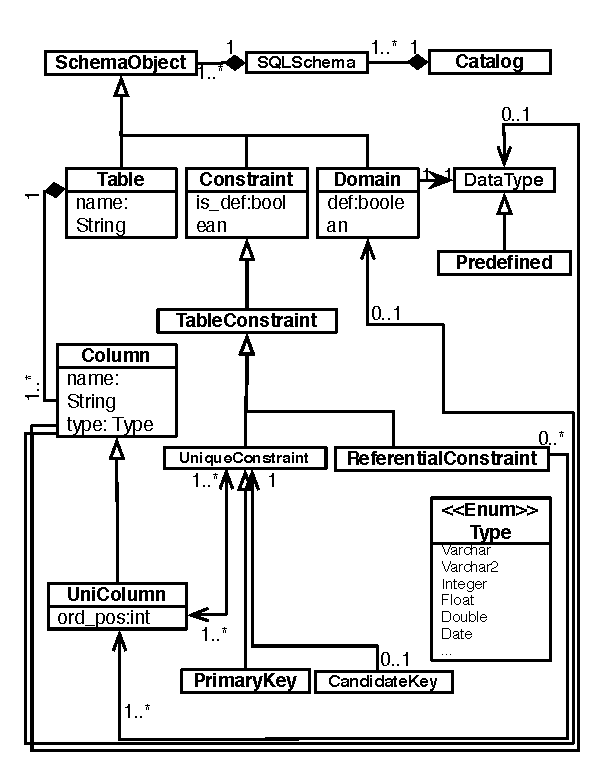
\includegraphics[scale=0.75]{figuras/SQL92Novo}
\caption{SQL meta-model (simplified excerpt).}
\label{fig:sql_metamodel}
\end{figure}

\begin{itemize}

\item \textbf{Rule R1:} Tables that were found in any SQL statement (Insert, Select, Update or Delete) as either source or target clauses (From, Set, Into, and so on) are represented by an instance of the meta-classe Table, see Figure~\ref{fig:sql_metamodel};

\item \textbf{Rule R2:} The columns that are identified by means of the parser or by the database metadata in the SQL statements are created in the corresponding tables. These tables have previously been created through the application of \textbf{R1}. Those columns are represented by the meta-classe Column, see Figure~\ref{fig:sql_metamodel}.

\item \textbf{Rule R3:} The data type associated with each column was deduced through the database metadata. Therefore, for the columns that have previously been created through the application of \textbf{R2}, are now updated with their specific type, see the meta-Enumeration named Type in Figure~\ref{fig:sql_metamodel}.

\item \textbf{Rule R4:} The constraint of columns  was also deduced through the database metadata. As result, for the columns that have previously been created through the application of \textbf{R2}, at least one should be flagged as primary key. Thus, if a column is primary key then an instance of the meta-classe PrimaryKey is instantiated. 

\item \textbf{Rule R5:} Foreign key that were found in the database metadata are represented by an instance of the meta-classe ReferentialConstraint, see Figure~\ref{fig:sql_metamodel}.

\end{itemize}

Upon finishing the instantiation of both PSMs (Java model and SQL model), the next two steps consist of transforming them into KDM, which represent the same information but in a platform-independent manner. To do so, two steps must be carried out: (\textit{i}) \textit{JavaModel2KDMCode}, and (\textit{ii}) \textit{SQLModel2KDMData}, Figure~\ref{fig:activity_diagram} steps \circled{\textbf{E}} and \circled{\textbf{F}}, respectively. %The JavaModel2KDMSource transformation is carried out on instances of Java meta-mode (Figure~\ref{fig:java_metamodel}), and produces a corresponding model based on the KDMSource meta-model. Similarly, the SQLModel2KDMData transformation is carried out on instances of SQL meta-model (Figure~\ref{fig:sql_metamodel}), and produces a corresponding model based on the KDMData meta-model. 
As stated in Section~\ref{subsec:KDM} KDM contains severals meta-models, but herein we are only interested in the Code meta-model, which represents the code elements of a program and their associations and in the Data meta-model which defines a set of meta-model elements whose purpose is to represent organization of data in the existing software system. A briefly overview of both meta-models KDMCode and KDMData are depicted in Figure~\ref{fig:KDMSOurce} and~\ref{fig:KDMDATA}. 


\begin{figure}[!h]
\centering
  % Requires \usepackage{graphicx}
  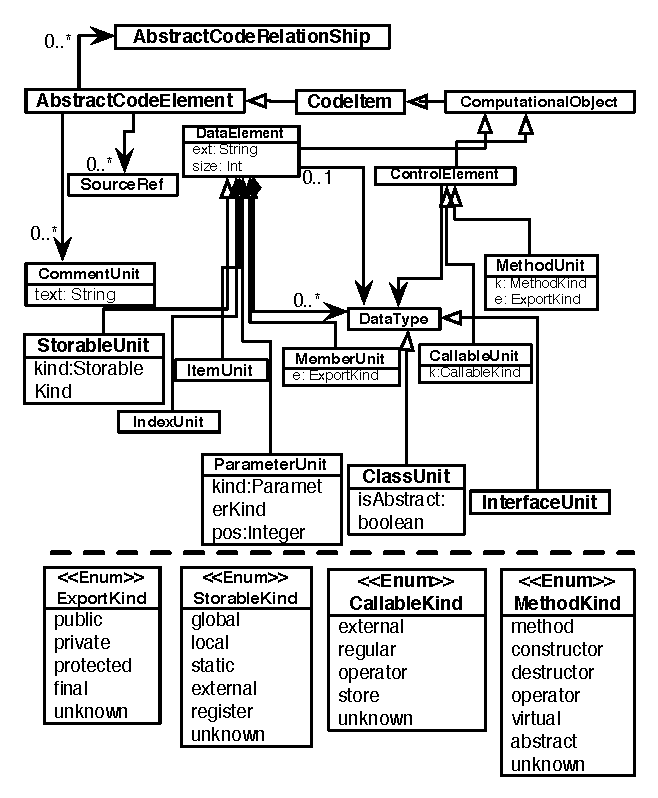
\includegraphics[scale=0.70]{figuras/KDM-Program-Layer}
\caption{KDM code meta-model (simplified excerpt).}
\label{fig:KDMSOurce}
\end{figure}

%A briefly description of both KDMSource and KDMData are depicted in Figure~\ref{fig:KDMSOurce} and~\ref{fig:KDMDATA}.

 Our approach uses ATL (ATLAS Transformation Language)~\cite{Jouault200831} to realize model-to-model transformations. In Listing~\ref{list:KDMSource1} is depicted a chunk of code related to the transformation \textit{JavaModel2KDMCode}, i.e., step \circled{\textbf{E}}. Notice that the \textit{JavaModel2KDMCode} is carried out on instances of Java meta-mode (Figure~\ref{fig:java_metamodel}), and produces a corresponding model based on the KDMSource meta-model, see Listing~\ref{list:KDMSource1} in lines 1 and 2. ATL is based in \textit{rules}. Therefore, we have defined a set of rules to transform each meta-classe of the Java meta-model (Figure~\ref{fig:java_metamodel}) to a instance of KDMCode. 


Lines  3-8 show a rule to transform instance of packages from the source (Java meta-model) to packages of the target meta-model (KDMCode), by keeping the same name. Lines 10-20 illustrate a transformation rule responsible to transform from the Java meta-model instance of class (\textit{ClassDeclaration}) and its methods (\textit{MethodDeclaration}) to \textit{ClassUnit} and \textit{MethodUnit} of the target KDMCode meta-model.


%A briefly description of the meta-model of KDMSource is depicted in Figure~\ref{fig:KDMSOurce}.

\begin{lstlisting}[caption=Chunk of JavaModel2KDMCode, label=list:KDMSource1, frame=lrtb, basicstyle=\tiny]
module JavaModel2KDMSource;
create OUT:KDMSource from IN:JavaModel;
rule Package{ 
  from
     ps:JavaModel!Package 
  to
     pt:KDMSource!Package( 
	  name<-ps.name)
} 
rule Class{ 
  from
    cs:JavaModel!ClassDeclaration(
          cs.ownedOperation->notEmpty())
  to
       ct:KDMSource!ClassUnit(
        name<-cs.name,
        package<-cs.package,
        methodUnit<-opeLst
   ),
   opeLst:distinct JavaModel!MethodDeclaration foreach
(oper in cs.methodUnit.asSequence()) (name<-oper.name)
}
[...]
}
\end{lstlisting}


\begin{figure}[!h]
\centering
  % Requires \usepackage{graphicx}
  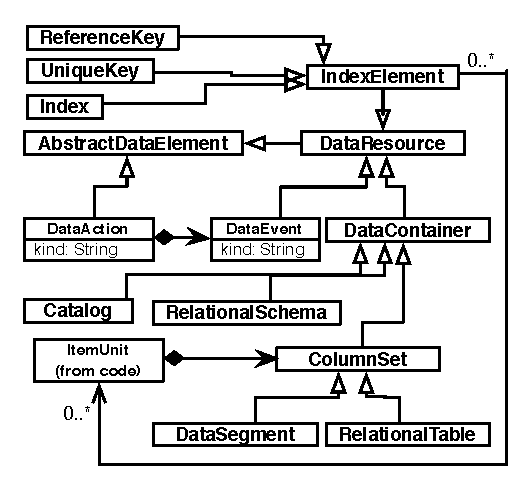
\includegraphics[scale=0.78]{figuras/KDM-Data-Layer}
\caption{KDM data layer (simplified excerpt).}
\label{fig:KDMDATA}
\end{figure}

The second transformation \textit{SQLModell2KDMData} is carried out on instances of SQL meta-mode (Figure~\ref{fig:sql_metamodel}), and produces a corresponding model based on the KDMData meta-model (Figure~\ref{fig:KDMDATA}), see Listing~\ref{list:KDMData} in lines 1 and 2. Lines 4-12 describe a rule to transform the \textit{SQLSchema} from the source (SQL meta-model) to \textit{RelationalSchema} of the target meta-model (KDMData), by copying the name and the references of all tables. After, in lines 13-21 are described a rule to transform the \textit{Table} from the source (SQL meta-model) to \textit{RelationalTable} of the target meta-model (KDMData), by copying the name and keeping all columns of such \textit{Table}. In lines 22-28 show a rule to transform \textit{Column} and its type from the source meta-model to \textit{ColumnsSet} of the target meta-model. Finally, in lines 30-34 the types of the columns are identified.

\begin{lstlisting}[caption=Chunk of SQLModel2KDMData, label=list:KDMData, frame=lrtb, basicstyle=\tiny]
module SQLModel2KDMData;
create OUT:KDMData from IN:SQLModel;

rule SQLSchema2RelationalSchema {
	from 
		t: SQLModel!SQLSchema
	to
		r: KDMData!RelationalSchema (	
			name <- t.name,
			relationalTable <- t.table
		)
}
rule Table2RelactionalTable {
	from
		t: SQLModel!Table
	to
		r: KDMData!RelationalTable (
			name <- t.name,
			ownedAttribute <- t.columns
		)
}
rule Column2ColumnSet {	
	from
		t: SQLModel!Column (t.oclIsTypeOf(SQLModel!Column))
	to
		r: KDMData!ColumnSet (
			name <- t.name,
			type <- typeDATA
		),
		typeDATA : MM2!PrimitiveType(
			name <- t.itemUnit.first().type.name,
			type <- t.item.primitiveType
		)
}
[...]
}

\end{lstlisting}

\subsection{Reestructuing} % (fold)
\label{sub:restructuing}


The goal of this phase is to analysis the models created earlier to modernize automatically the legacy system into services, i.e., RESTFull operations. Therefore, in this phase is carried out an algorithm which takes as input both models KDMCode and KDMData - then four steps are conducted to create a set of services. The Algorithm 1 presents how the services are create, more information related to the steps are as follows:

%Services are entities that are either annotated with @Path or have at least one method annotated with @Path or a request method designator, such as @GET, @PUT, @POST, or @DELETE. 

Services are entities that are either annotated with @Path or have at least one method annotated with @Path or a request method designator, such as @GET, @PUT, @POST, or @DELETE. Thus, firstly, it is necessary to create entities with the information identified earlier. In other words, one must to transform all identified embedded SQL code (the tables, columns and even the relationship), which are now represent by the metaclasses of the KDMData to the correct metaclasse of the KDMCode. This is carried out by the step \circled{\textbf{G}}, see Figure~\ref{fig:activity_diagram}. Lines 2 of the Algorithm 1 depicts a loop which is executed for each meta-classe \textit{RelationalTable} belonging to the metamodel KDMData. After, in line 3, the function \textit{createClassUnit} is called. This function gets the meta-attributes name of the \textit{RelationalTable} and then create an instance of the meta-classe \textit{ClassUnit}. \textit{ClassUnit} is a meta-class that represents user-defined classes in object-oriented languages~\cite{5328801}. In line 4, the function \textit{createDataElement} is executed. This function obtains the all columns of the \textit{RelationalTable} and then create an instance of the meta-classe \textit{DataElement} which represent attributes in the KDM. In line 5 the function \textit{createMethodUnit} is carried out. This fuction is similar to the last one, however, instead of attributes, \textit{gets} and \textit{sets} are created. These methods are represented by instances of the meta-classe \textit{MethodUnit} which represents member functions owned by a ClassUnit.

\begin{figure}
\centering
  % Requires \usepackage{graphicx}
  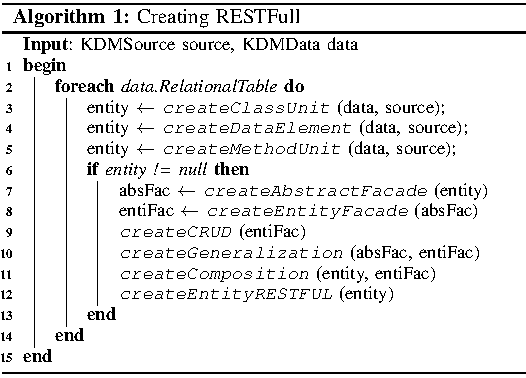
\includegraphics[scale=0.78]{figuras/alg}
\end{figure}

Afterwards, the services must be indeed created. As for we used the Facade Pattern~\cite{Gamma1994}, see Figure~\ref{fig:activity_diagram} step \circled{\textbf{H}}. The Algorithm 1, lines 7-12 depicts how the services are created. Firstly, in line 7 the function \textit{createAbstractFacade} is called to instantiate a meta-classe \textit{ClassUnit} which represents the \textit{AbstractFacade} of each entity. Secondly, in line 8 shows the function \textit{createEntityFacade} that is also an instance of the \textit{ClassUnit} which now represents the service. Thirdly, in line 9 the function \textit{createCRUD} depicts that for each entity four methods are create, i.e., create, retrieve, update and delete. Fourthly, the functions \textit{createGeneralization} and \textit{createComposition} in line 10 and 11 depict that relationships of generalization and composition are created. Finally, in line 12 the function \textit{createEntityRESTFUL} is carried out. It is responsible to inject request method designator (@GET, @PUT, @POST, or @DELETE), see Figure~\ref{fig:activity_diagram} step \circled{\textbf{I}}.

In the last step a set of configuration files are created. These files store project configuration data or settings, see Figure~\ref{fig:activity_diagram} step \circled{\textbf{J}}.

\subsection{Forward Engineering - FE} % (fold)
\label{sub:forward_engineering}

Forward Engineering (FE) is the process of bringing high-level abstractions to physical implementation of a system[ref]. This phase starts with the step \circled{\textbf{K}}, see Figure~\ref{fig:activity_diagram}. In this phase the restructured KDM model obtained in the \textit{Reestructuring} phase now is transformed to an instance of Unified Modeling Language (UML)~\cite{OMG}. 

\begin{lstlisting}[caption=Chunk of KDM2UML, label=list:KDM2UML, frame=lrtb, basicstyle=\tiny]
module KDM2UML;
create OUT:UML from IN:KDM;

rule Package2Package {
	from 
		t: KDM!Package
	to
		r: UML!Package (	
			name <- t.name,
			[...]
		)
}
rule ClassUnit2Class {
	from
		t: KDM!ClassUnit
	to
		r: UML!Class (
			name <- t.name,
			ownedAttribute <- t.memberUnit,
			ownedOperation <- t.methodUnit,
			[...]
		)
}
rule MemberUnit2Property {
	from
		t: KDM!MemberUnit
	to
		r: UML!Property (
			name <- t.name,
			type <- t.ownedType,
			[...]
		)
}
rule MethodUnit2Operation {	
	from
		t: KDM!MethodUnit (t.oclIsTypeOf(SQLModel!MethodUnit))
	to
		r: UML!Operation (
			name <- t.name,
			return <- returnDATA
			[...]
		),
		returnDATA : MM2!ReturnType(
			name <- t.itemUnit.first().type.name,
			type <- t.item.primitiveType
		)
}
[...]
}
\end{lstlisting}

Due space limitation in Listing~\ref{list:KDM2UML} is depicted just a chunk of the code written in ATL which is responsible to realize such transformation. In lines 4-11 are described a rule to transform the \textit{\texttt{Package}} from the source (KDM) to \textit{\texttt{Package}} of the target meta-model (UML). Lines 13-23 depict a rule to transform all \textit{\texttt{ClassUnit}} from the source (KDM) to \textit{\texttt{Class}} of UML. This rule copies the name of the \textit{\texttt{ClassUnit}}, all \textit{\texttt{memberUnit}}, all \textit{\texttt{methodUnit}} and also the relationships among the classes. After transform \textit{\texttt{ClassUnit}} to \textit{\texttt{Class}}, all \textit{\texttt{memberUnit}} and \textit{\texttt{methodUnit}} must be transformed. The former, is depicted in rule \textit{\texttt{MemberUnit2Property}}, lines 24-33. In lines 28-31 the \textit{\texttt{Property}}'s name and type are assigned. The latter, is shown in rule \textit{\texttt{MethodUnit2Operation}} in which lines 38-47 depict how all \texttt{MethodUnits} are properly transformed to \texttt{Operation}.  

  and etc are set  are shown a rule that transforms all \textit{memberUnit}, which represents in KDM both association and attributes,      


  activity Refine Model, which in- cludes the Analysis and Design disciplines of software devel- opment process. This activity is essential for the develop- ment of the new application, since the OO model generated in the RE needs to be refined and complemented according with new requirements and specifications not performed by code generation.

% subsection forward_engineering (end)

 %the step \circled{\textbf{G}} is carried out, see Figure~\ref{fig:activity_diagram}. This step is responsible to transform all identified embedded SQL code, which is now represented by the metaclasses of the KDMData to the correct metaclasse of the KDMCode.  


%Firstly, in order to create services it is necessary to transform the identified embedded SQL code into entities in  	

%Firstly, the \ref{fig:activity_diagram} step \circled{\textbf{G}} is carried out. Here 



%The goal of this phase is to apply a set of rules into the models created earlier, i.e., both KDMCode and KDMData, in order to automate the devising of services. 


 %the models created previously in order to automate the devising of services. A set of rules are applied into the models created earlier in order to automate the devising of services. 
\section{\uppercase{Proof-of-concept implementation}}\label{sec:proof_of_concept_implementation}

We devised a proof-of-concept implementation named Modernization-Integrated Environment (MIE). 


%In this section is shown the architecture of the ProLine-RM as well as an description of its components. 
In Figure~\ref{fig:architecture} is depicted the architecture of MIE. As shown in this figure, we devised it on the top of the Eclipse Platform and used both Java and Groovy as programming language. Moreover, we used Eclipse Modeling Framework (EMF)\footnote{http://www.eclipse.org/modeling/emf/} to create the SQL model, the SOA model and to reutilize the UML model. MoDisco is used by the infrastructure since it provides an
\textbf{A}pplication \textbf{P}rogramming \textbf{I}nterface - (API) to easily access the KDM model. 

\begin{figure}[!h]
\centering
  % Requires \usepackage{graphicx}
 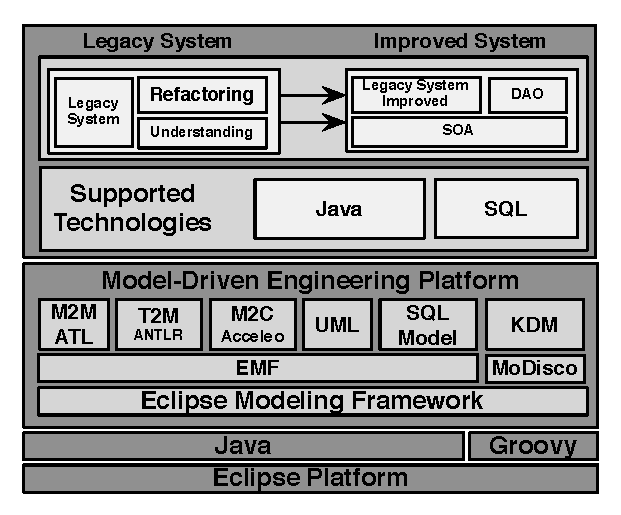
\includegraphics[scale=0.6]{Figuras/Arquitetura_da_Ferramenta}
\caption{Architecture of Modernization-Integrated Environment.}
\label{fig:architecture}
\end{figure}


\textbf{A}Nother \textbf{T}ool for \textbf{L}anguage \textbf{R}ecognition -  (ANTLR) is used herein to create parsers to obtain information related to the legacy system's artifacts. Therefore, two parser were developed: (\textit{i}) the first takes as input a Java grammar and generates as output an AST and (\textit{ii}) the second parser is an extension of the first one to identify SQL embedded in the legacy system's source code, i.e., it takes as input a Java source-code and generates as output an AST which contains informations such as, tables, columns, primary keys, etc. Then, to transform these ASTs in PSMs we used an API provided by EMF. Afterwards, all the transformations M2M are done by \textbf{A}tlas \textbf{T}ransformation \textbf{L}anguage - ATL, which provides ways to produce a set of target models from a set of source models. Therefore, ATL is used to transform the PSMs to conform the KDM specification and to transform the improved KDM to an UML that represents the target systems. 

Finally, in order to transform this last model in a set of physical artifacts (source code), i.e., model-to-code transformations, Acceleo was used, which is based on textual template approach. A template can be thought of as the target text with holes for variable parts. The holes contain metacode which is run at template instantiation time to compute the variable parts. Furthermore, we have used Java Persistence API (JPA) 2.0 to deal with the way relational data is mapped to Java objects. Similarly, RESTful API have been used to implements SOA artifacts. 

\section{\uppercase{Related Work}}\label{sec:related_work}

Several research works have been proposed by the academic community are related to the concepts discussed in this paper.

Modernization of Legacy Web Applications into Rich Internet Applications [ref] proposes a approach for systematic and semiautomatic modernization of legacy Web applications in rich interfaces applications. In this process, the MDD principles are applied and the use of ADM specifications for the generation of rich interfaces from the source code of navigation and presentation layers of legacy web applications. The proposed approach differs from this work by having a more general purpose and are not intended to only a single type of applications, such as Web applications. In addition, the proposed approach offers the possibility to use the database in the process of reengineering.

Model-Driven Reengineering of Database [ref] presents a process to perform relational databases reengineering. The process is conducted through of repeated model transformations and divided into the stages of extraction and contextualization. In the extraction stage, a PSM is obtained from the database structure. In the contextualization stage, a PIM is generated from the PSM. As a result of the process, there are entity-relationship models and class diagrams. The proposed approach differs from this work by using object-relational mapping frameworks and metaprogramming techniques to obtain a model of the database structure, rather than using several model transformations, resulting in a more simple and faster way to extract knowledge from the database.


\section{\uppercase{Case Study}}

This section presents a case study to validate the proposed approach by applying it to a real-life legacy information system. As stated in Section~\ref{sec:proof_of_concept_implementation} we devised a proof of concept tool which implements our approach. Notice that the case study was carried out following the protocol for planning, conducting and reporting case studies proposed by Brereton \textit{et al}. in~\cite{case-study-template-2008} improving the rigor and validity of the study. The next subsections show more details about the main phase defined in this protocol, such as: background, design, case selection, case study procedure, data collection, analysis and interpretation and validity evaluation.


\subsection{Background} % (fold)
\label{sub:background_case_study}

According to the protocol proposed by Brereton \textit{et al}. in~\cite{case-study-template-2008} firstly it is needed to identify previous research on the topic. Hence, in Section~\ref{sec:related_work} we stated some researches related to modernize legacy system by using both ADM and MDD. Particularly, the approach herein described aims to identify embedded SQL statement in a legacy system and then by means of the ADM approach model transformations are realized until obtain a new system - now reestructured to use services with RESTFULL. As result, the object of this study is that the proposed approach identifies the embedded SQL statements in a legacy system, and the purpose of this study is the evaluation of the approach herein described related to its effectiveness and efficiency.

Therefore, taking into account the objects and purpose of the study, it was defined two research questions, as follows: 

\begin{itemize}
	\item \textbf{RQ$_1$}: Can the proposed approach obtain embedded SQL statement from legacy systems to effectively create services by using RESTFULL?
	\item \textbf{RQ$_2$}: Is the proposed approach efficient as compared to the classic life cycle of the software? 

	to be scaled to any legacy system?
\end{itemize}

The former question, \textbf{RQ$_1$}, verifies if the approach can obtain embedded SQL statement in a legacy system. In addition, \textbf{RQ$_1$} also assesses whether the identified SQL statements can be effectively transformed to services. The latter question, \textbf{RQ$_2$} aims to verify the efficiency of the proposed approach when compared to the classic life cycle of the software.

\subsection{Design} % (fold)
\label{sub:design_case_study}

The described case study consist of a single case~\cite{citeulike:598898}, i.e., it focuses on a single legacy system. To assess the effectiveness of the proposed approach through the \textbf{RQ$_1$}, we chose to use two measures, they are: (\textit{i}) precision and (\textit{ii}) recall. These measures are used because precision can be seen as a measure of exactness or fidelity, whereas recall is a measure of completeness. In our context, precision illustrates the amount of relevant recovered embedded SQL statement within the set of recovered SQL statement in a legacy system. A SQL statement is considered relevant if this statement faithfully represents SQL operations of the legacy system in the real world. Recall represents the amount of relevant recovered embedded SQL statement of the total of relevant SQL statement (recovered and not recovered) that depict the whole SQL operations of the legacy system.

As for answering \textbf{RQ$_2$} we applied empirical estimation model according to Software Equation~\cite{Putnam:1991:MER:574087}, see Equation~\ref{eq:effort}. 

\begin{equation}
  E = [LOC * B^{0.333}/P]^3 * (1/t^4)
  \label{eq:effort}
\end{equation}

where:

E = effort in person-months or person-years 

t = project duration in months or years LOC = lines of code

B = special skill factor

P = productivity parameter


\subsection{Case Selection} % (fold)
\label{sub:case_selection}

In this section is described the suitable case that was chosen to be studied. Some criteria were applied to select the suitable case, as follows: (\textit{i}) it must be an enterprise system, (\textit{ii}) it must be a Java-based system, (\textit{iii}) it must be a legacy system and (\textit{iv}) it must be of a size not less than 10 KLOC. After applying these criteria we chose ProgradWeb\footnote{https://progradweb.ufscar.br/progradweb/} of Federal University of S\~ao Carlos (UFSCar). ProgradWeb is an academic system on the Web for managing information about teachers, students and undergraduate programs of UFSCar. 

The original architecture of the system was developed using Java Servlets and web pages in the Java Server Pages (JSP) language. The system runs on a server configured with Apache Tomcat\footnote{http://tomcat.apache.org/} and connects with a PostgreSQL database\footnote{http://www.postgresql.org/}, using the API Java Database Connectivity (JDBC). However, over time and the appearance of new requirements, the system maintenance became expensive, requiring its reengineering.

\subsection{Case Study Procedure} % (fold)
\label{sub:case_study_procedure}

In this section is shown how the execution of the study was planned. Notice that the execution was aided by the tool developed to support the proposed approach, see Section~\ref{sec:proof_of_concept_implementation}. The case study was carried out in a machine with an Intel Core I5 CPU 2.5GHz, 4GB of physical memory running Mac OS X 10.8.4. 

As stated in Section~\ref{sec:proposed_approach} the approach proposed herein starts with the RE. Firstly, discovering of knowledge must be carried out. As described earlier two parser are executed to obtain this knowledge: (\textit{i}) the first parser takes as input the ProgradWeb's source-code and generates as output an AST and (\textit{ii}) the second one is an extension of the first one; and its aims is to identify SQL embedded in the legacy system's source-code, i.e., it takes as input a Java source-code and generates as output an AST which contains informations such as, tables, columns, primary keys, etc. Secondly, the ASTs obtained are transformed in two PSMs, the Java PSM and the SQL PSM. Such transformations are executed by using an API provided by EMF. Thirdly, these PSMs are transformed to PIMs to be in conform to the KDM standardization, i.e., the Java model to KDM Code and SQL model to KDM Data. They are transformed by means of rules written in ATL. 


By using the KDM models obtained the next phase starts. in this phase is carried out an algorithm which takes as input both models \texttt{KDMCode} and \texttt{KDMData} - then four steps are conducted to create a set of services, see Algorithm 1. First, entities are created in the KDMCode (\texttt{ClassUnit}, \texttt{DataElement} and \texttt{MethodUnit}) by using the information of the KDMData (\texttt{RelationalTable}, \texttt{ColumnSet}). Second, services (CRUDs) are created by using the design pattern Facade~\cite{Gamma1994}.

The FE is started with the new KDM metamodels. ATL is also used in this phase to transform the KDM metamodel into both UML and SOA models. Finally, in order to transform these last models into physical artifacts (source-code) model-to-code transformations was applied. This is performed by mapping context models using a template-based approach to a corresponding
programming language and automatically generating the implementation.

After carrying the described approach, the new ProgradWeb was obtained. Then all embedded SQL statement, the created entities and the created services are collected according to the data collection plan. After that, the data collected previously is analysed and interpreted to draw conclusion to answer the research questions. Section x presents more information related to the results obtained from this case study.

\subsection{Data Collection} % (fold)
\label{sub:data_collection}

According to the protocol proposed by Brereton \textit{et al}. in~\cite{case-study-template-2008} the data to be collected and the data sources must be defined before starting the execution of the case study to ensure the future repeatability.



\begin{table}
	
\begin{tabular}{|c|c|c|}
\hline 
\multirow{8}{*}{\begin{sideways}
RE
\end{sideways}} & Steps & Time\tabularnewline
\cline{2-3} 
 & Parser source-code & 9'\tabularnewline
\cline{2-3} 
 & Parser Embedded SQL & 12'\tabularnewline
\cline{2-3} 
 & Create JavaModel & 7'\tabularnewline
\cline{2-3} 
 & Create SQLModel & 16'\tabularnewline
\cline{2-3} 
 & JavaModel\_2\_KDMSource & 11'\tabularnewline
\cline{2-3} 
 & SQLModel\_2\_KDMData & 7' 35''\tabularnewline
\cline{2-3} 
 & \cellcolor{gray!25}TOTAL Phase & \cellcolor{gray!25}62' 35''\tabularnewline
\hline 
\multirow{6}{*}{\begin{sideways}
Reestructuring
\end{sideways}} & Steps & Time\tabularnewline
\cline{2-3} 
 & Create Entities & 15'\tabularnewline
\cline{2-3} 
 & Apply Facade Pattern & 9'\tabularnewline
\cline{2-3} 
 & Create WebService & 10'\tabularnewline
\cline{2-3} 
 & Create Configuration Files & 2'\tabularnewline
\cline{2-3} 
 & \cellcolor{gray!25}TOTAL Phase & \cellcolor{gray!25}36'\tabularnewline
\hline 
\multirow{6}{*}{\begin{sideways}
FE 
\end{sideways}} & Steps & Time\tabularnewline
\cline{2-3} 
 & KDM\_2\_UML & 13'\tabularnewline
\cline{2-3} 
 & UML\_2\_JavaModel & 14' 50''\tabularnewline
\cline{2-3} 
 & UML\_2\_RestModel & 6' 27''\tabularnewline
\cline{2-3} 
 & Generate Source-Code & 5' 39''\tabularnewline
\cline{2-3} 
 & \cellcolor{gray!25}TOTAL Phase & \cellcolor{gray!25}40' 33''\tabularnewline
\hline 
\multicolumn{2}{|c|}{\cellcolor{gray!25}TOTAL Modernization} & \cellcolor{gray!25}2 hours and 30'\tabularnewline
\hline 
\end{tabular}

\end{table}

\begin{table*}
\centering	
\begin{tabular}{|>{\centering}p{1.2cm}|>{\centering}p{1.6cm}|>{\centering}p{1.3cm}|>{\centering}p{1.5cm}|>{\centering}p{1.9cm}|>{\centering}p{2cm}|>{\centering}p{1.4cm}|>{\centering}p{1.4cm}|}
\hline 
SQL Statement & Identified Statements (IS) & Identified Table (IT) & Created Relevant Services (CrRS) & Created Non-Relevant Services (CrNRS) & Non-Created Relevant Service (NCrRS) & Precision $\frac{CrRS}{CrRS + CrNRS}$ & Recall $\frac{CrRS}{CrRS + NCrRS}$\tabularnewline
\hline 
\hline 
Select & 382 & 67 & 67 & 0 & 1 & 100\% & 98.52\%\tabularnewline
\hline 
Update & 83 & 40 & 38 & 2 & 3 & 95\% & 97.56\%\tabularnewline
\hline 
Delete & 33 & 20 & 15 & 5 & 2 & 75\% & 88.23\%\tabularnewline
\hline 
Insert & 37 & 28 & 27 & 1 & 1 & 96.42\% & 96.42\% \tabularnewline
\hline 
Total & 535 & 155 & 147 & 8 & 7 &  & \tabularnewline
\hline 
Mean & 133.75 & 38.75 & 36.75 & 2 & 1.75 & 91.60\% & \tabularnewline
\hline 
\end{tabular}

\end{table*}


% subsection data_collection (end)
% subsection design (end)
% subsection background (end)

%KDM-Program-Layer
%\begin{itemize}

%\item Rule 1: Each package is transformed to instances of the meta-classe Package;

%\item Rule 2: Numbers and Strings are transformed to instances of the meta-classe PrimitiveType;

%\item Rule 3: 

%\item Rule 4: Ifs are transformed to instances of the meta-classe IfStatement;

%\item Rule 5: 

%\item Rule 6: Methods are transformed to instances of the meta-classe MethodDeclaration;

%\end{itemize}       





%\begin{small}
%\begin{verbatim}
%import java.sql.*;

%public class Entity {
%	private String sql1 = "select * from table1";

%}
%Begin
  %   Writeln('Hello World!!');
% End.
%\end{verbatim}
%\end{small}

%AST database model that illustrates informations related to database used in the legacy system, see Figure 2(A). Similarly, this model is also represented by an AST, the only difference is that it represents syntactic structure of database instead of Java source code.


%Java metamodel which is the reflection of the Java language, as defined in version 3 of ``Java Language Specification'' from Sun Microsystems. This Java metamodel contains 126 metaclasses  

%



%we had to use two parsers to obtain information related to these artifacts. The former parser is responsible to takes as input the legacy system's source-code and then builds a data structure, e.g.,  



 %giving a structural representation of the input, checking for correct syntax in the process. The parsing may be preceded or followed by other steps, or these may be combined into a single step. The parser is often preceded by a separate lexical analyser, which creates tokens from the sequence of input characters; alternatively, these can be combined in scannerless parsing. Parsers may be programmed by hand or may be (semi-)automatically generated (in some programming languages) by a tool.  

%\circled{\textbf{A}}





\section*{\uppercase{Acknowledgements}}

\noindent 

\vfill
\bibliographystyle{apalike}
{\small
\bibliography{example}}

\vfill
\end{document}

